%%% Time-stamp: <2015-04-15 00:55:14 sunthar>

%%% $Log:$

%\documentclass[11pt
\documentclass[seminar,twoside]{iitbreport}



%% Selectively comment out sections that you want to be left out but
%% maintaining the page numbers and other \ref
\includeonly{%
  intro/introduction,
  lit/literature,
  expt/experimental,
  rnd/results,
}

%%% Some commonly used packages (make sure your LaTeX installation
%%% contains these packages, if not ask your senior to help installing
%%% the packages)

\usepackage{tabularx}
\usepackage{booktabs}
\graphicspath{{expt/}}
\usepackage{xcolor}
\hypersetup{
  colorlinks,
  linkcolor={black!50!black},
  citecolor={black!50!black},
  urlcolor={black!80!black}
}


%%% Macro definitions for Commonly used symbols
\newcommand{\etas}{\ensuremath{\eta_{\mathrm{s}}}}
\newcommand{\Rey}{\ensuremath{\mathrm{Re}}}
\newcommand{\avg}[1]{\ensuremath{\overline{#1}}}
\newcommand{\tenpow}[1]{\ensuremath{\times 10^{#1}}}

\newcommand{\pder}[2]{\ensuremath{\frac{\partial#1}{\partial#2}}}


% Referencing macros
\newcommand{\Eqref}[1]{Equation~\eqref{#1}}
\newcommand{\Tabref}[1]{Table~\ref{#1}}
\newcommand{\Figref}[1]{Figure~\ref{#1}}
\newcommand{\Appref}[1]{Appendix~\ref{#1}}



\begin{document}
\title{Performance and Power Management of Virtualized Platform}
\author{
{Under the guidance of\\
Prof Varsha Apte}\\ \vfill Abhishek Pratap Singh \\ 143050077\\}
%\date{\today}

\degree{Master of Technology}
\dept{Computer Science}
%\monthyear{May 2016}

%\makecoverpage
\maketitle

\begin{abstract}
This report is about what is virtualization and power management in virtualized platforms.
There are many organizations and communities working in this field but Xen and KVM are
milestone in this field. Xen started an open source project to host multiple guest OSes
with an approach of paravirtualization. The interesting thing about KVM is it is integrated
with Linux kernel so its development happening with development of Linux kernel. Virtualization 
has performance issue so hardware support was the need of virtualization.
Nowadays Intel and AMD provides hardware support. KVM provides virtualization using
this hardware support. “Which virtualization platform is best” is hot topic, there is a need
of regular comparison among all virtualization options to find out which one is best in a
particular situation or requirement. This report describes about comparison of virtualization 
platform as well. Virtualization provides Consolidation and VM migration strategy to
power management but this facility(virtual platform) comes with complication to manage
power in virtualized platform this report describes how to deal with power management
in virtualized platform. In last section focus on coordination among different but simultaneous 
power management plans, and some improvement in scheduler to make fair cpu
capacity allocation during frequency scaling.
\end{abstract}

\pagenumbering{roman}
\tableofcontents

\setcounter{page}{1}
\pagenumbering{arabic}
\renewcommand{\thesection}{\arabic{section}}
\begingroup
\let\cleardoublepage\clearpage
%\listoftables
%\listoffigures

%\cleardoublepage
\setcounter{page}{1}
\pagenumbering{arabic}

%
\chapter{Introduction}


This document contains commonly used essential templates to write a
\LaTeX\ document. This document is to be used along with the files and
folders provided. Writing a \LaTeX\ document is very simple.  Often
students need only very simple constructs.  This document shows
certain essential features that almost all technical report writing
requires. Please consult the PDF file for the output of the document,
and then look at the corresponding \LaTeX\ file to reproduce it.  The
document illustrates the following constructs
\begin{itemize}
\item Unnumbered and Numbered Lists
\item Equations
\item Defining short macros for frequently used symbols
\item Bibliography
\item Figures
\item Tables
\end{itemize}

The normal procedure for compiling a \LaTeX\ document that contains
bibliographic entries is to follow the following steps
\begin{enumerate}
\item \verb|pdflatex mainrep|
\item \verb|bibtex mainrep|
\item \verb|pdflatex mainrep|
\item \verb|pdflatex mainrep|
\end{enumerate}
In the above example \verb|mainrep| is the main \LaTeX\ file.


\section{First section of this chapter}

This is the first chapter, which resides in a directory (folder)
intro. Each chapter can contain \verb|section|, \verb|subsection|
and so on.

\subsection{Equations and Math symbols}


Equations should be set in a separate mode.  For details on getting
various types of aligned equations, consult the \AmS-\LaTeX\
documentation \verb|amsldoc.pdf|. Simple equations are set as
\begin{equation}
\label{eq:sinx}
\int \mathrm{d}x \; \cos x =  \sin x
\end{equation}
Equation~\eqref{eq:sinx} is the integral of the cosine
function. Mathematical symbols must always be put inside \verb|$$|,
when they appear outside a math environment (such as \verb|equation|,
\verb|align|, \verb|gather|, etc).  The symbol ``ex'' must be written as
$x$ and not as x.  

Another commonly used construct for equations is the \verb|align|
environment to align several equations along a vertical line. It is
usually the $=$ sign across which the alignment is done.  The
point of alignment for each equation is specified using the ampersand symbol 
\begin{align}
a &= b  \\
a + e + f + g & = m + n + z \\
x + 2 & = x^{3} + 3 x^{2} + 2 x + 5
\end{align}

\subsection{Commonly used Symbols}
For mathematical symbols it is very convenient to define frequently
used symbols as a short macro. For example if you are to be using the
symbol $\eta_{\mathrm{s}}$ frequently it is convenient to define it in
as:\\
\verb|\newcommand{\etas}{\ensuremath{\eta_{\mathrm{s}}}}| \\
in the preamble and to simply refer it to in the text as \etas\ or in
a mathematical equation as $\etas = \eta \, ( 1 + \phi)$.

%%% Local Variables: 
%%% mode: latex
%%% TeX-master: "../mainrep"
%%% End: 

%
\chapter{Literature Survey}

The bibliographic entries are to be kept in a file named
\verb|<something>.bib|. In this sample report we call it as
\verb|mylit.bib|. This file must be included without the \verb|.bib|
extension in the main file as: \verb|\bibliography{mylit}|.   Open the
file \verb|mylit.bib| to see the format in which the entries are
written. This is written in the Bib\TeX format. Most of the
bibliographic web pages (Scopus, ISI Web) and software (EndNote, etc)
allow you to export bibliographic entries in the Bib\TeX format.

Citations are referred in the text using \verb|\citet| command which produces
citations as though they are part of the text.  In order to say
somebody did this work as a part of a line use:
\verb|\citet{Batzri1973}|
have done extensive work on \ldots.  This will produce

\citet{Batzri1973} have done extensive work on \ldots


Alternately citations can appear in parenthesis.  The
command \verb|\citep{Batzri1973}| is used to automatically put the
citations in parenthesis.
  As an example consider the extensive work
done in the area of book writing \citep{Sackmann1995a,Boal2012}.

Conferences \citep{rich-mart92} or collection of work
\citep{Sackmann1995a} also have special entries.

It is also possible to cite thesis like this:
\citet{jariwala00,luding94} or just unpublished work from
\citet{SunHI03}. Some times there are unclassified bibliographic
entries which can be put under ``misc'' \citep{Smith99}.



%%% Local Variables: 
%%% mode: latex
%%% TeX-master: "../mainrep"
%%% End: 

%
\chapter{Materials and Methods}

\section{Including Figures}

Figures are conveniently included using postscript format.  If you are
generating a figure in a software, please check if the software
supports writing to a postscript or a PDF format. This format is loss
less vector format and with reproduce in any magnification without any
pixelation. Make sure to write it to an ``Encapsulated Post-script''or
.eps format.


\begin{figure}[tbp]
  \begin{center}
    
\includegraphics[width=0.7\textwidth]{profflow}
    \caption[Process flow sheet]{Process flow sheet of the
      experimental setup. The caption of the figure goes here. A
      shorter caption can be written in square brackets to identify it
      in the list of figures.}
    \label{fig:pfs}
  \end{center}
\end{figure}

Figures should be given a label and which can be used to refer to them
in the running text using \verb|\ref{}| command. Figure~\ref{fig:pfs}
describes the process flow sheet of the experimental set up used in
this report. The \Figref{fig:pfs} can also be refered by a short form notation
a pre-defined macro \verb"\Figref".



%%% Local Variables: 
%%% mode: latex
%%% TeX-master: "../mainrep"
%%% End: 

%\chapter{Results and Discussion}


\section{Including Tables}

Tables are to be used in a special environment so that they have a
Number, caption and appear in the list of tables.
Table~\ref{tab:samtab} is a sample table. In the case of tables, it is
a convention to write the caption above the table.  Note that in the
case of figures the caption appears below the figure.

\begin{table}[tbp]
  \begin{center}
    \caption{Physical properties of the materials used.}
    \label{tab:samtab}
    \begin{tabular}{ll}
      \toprule 
      Property & Value \\
      \midrule
      Particle Density, $\rho_{\mathrm{p}}$ & 2500 kg/m$^{3}$ \\
      Viscosity, $\eta_{\mathrm{s}}$& 1 $\times 10^{-3}$ Pa-s \\
      \bottomrule \\
    \end{tabular}
  \end{center}
\end{table}

%%% Local Variables: 
%%% mode: latex
%%% TeX-master: "../mainrep"
%%% End: 


\section {Introduction}
Data centers requires different servers and different application, all of them can
not run on same hardware without affecting each other, deploying separate 
hardware for each such server and application is very inefficient, costly and hard
to manage. Virtualization is very nice solution for this problem. This is simple one of 
motivations for virtualization Technology. Virtualization provides a platform
which create illusion to application or user that he is working with bare metal.

Virtualization have some property to ensure feasibility and fairness to Virtual machines 
1. Isolation if more than one VM running on a same physical machine then one
VM should not affect adversely the performance of others. 
2. Support to various type of operating systems 
3. Overhead to provide virtualization should be least \cite{xen}. 
Xen was released in 2003 by university of Cambridge computer laboratory.
When Xen was released hardware support for virtualization was not common, 
so Xen used paravirtualization approach to implement virtualization. 
In paravirtualization Xen patches host operating system source code and guest operating
system source code to create virtual platform. KVM also provides virtualization but it 
runs only on Linux systems but integration with Linux provides growth in
development with Linux kernel. KVM depends on hardware support made available by Intel
and AMD, and virtual machines run in guest mode of processor.\cite{kvm} In next section Comparison 
among Xen, KVM and other Virtualization technologies. Power Management in
Virtualized Platforms: In virtual platform access to hardware directly is not provided

normally. If direct access given to hardware then it creates some serious problems, eg. 
violation of isolation property and there will be no difference in privilege level of host
and guest. Challenges Related to Virtual Power Management: This report

focuses mainly on two Challenges 1. Inconsistency when different power management act
simultaneously in uncoordinated way. \cite{nostruggle} 2. When more than one VM running on a single
physical machine and all VM allocated some fixed credits, consider some VMs with
less credits running overloaded but physical machine is under loaded globally then DVFS
detects this global under load and reduce frequency. This reduction in frequency affects
adversely overloaded VMs \cite{dvfs}.
%{\bf Solution approches to solve above Challanges:} 
\section{Virtualization Technologies}
\subsection{Virtualization}
Virtualization is a way to creates illusion of hardware machine on which applications run without knowing it, 
but now virtualization supported by hardware 
because virtualization has an inherent problem of performance. To increase speed
of execution there are two simple ways to solve this either provide hardware support to
virtualization or make high performance hardware for host OS. first method is better than
second one because it reduces emulating overhead on hypervisor so its speed improves,
but in second way due to high performance effects of overhead becomes negligible. 
Virtualization provides independence on hardware, a server running on virtual machine can
replicate and migrate according to need, so maintenance of server farm has become very
easy and automatic. Live VM migration provides a way to use hardware efficiently in
terms of power in technical term it is known as consolidation.
\subsection{Xen}
Xen is first independent open source virtualiztion technique which uses paravirtualization. 
Xen purposed paravirtualization technique to implement virtual platform for guest
OSes. Hypervisor ensured isolation by multiplexing Guest OSes instead of processes.
In paravirtualization we need to modify some source code of host OS and guest
OS. x86 architecture is not virtualization-friendly 
so implementation of virtualization introduce performance degradation and increased complexity, 
to overcome this problem paravirtualization used to make it faster. 
Xen do not fully virtualized I/O devices, instead used an abstraction of devices which is quite similar to hardware. 
Xen hypervisor works at higher privilege level and provide interface between host and guest and 
validate communication between Guest OS and Hardware. There is special guest Dom 0 which controls all operation 
related to communication to network devices and I/O devices. 
Positive Points:
1. Address space swithes followed by complete TLB flush, to solve this problem code of XEN resides in 64 MB section in each adress space at Top position, 
so it prevent entire tlb flush.
2. To reduce overhead guest OS manages mapping of page tables.
To provide protection in page table Xen validates every update to page table by ensuring that (a) Page that Os want to map should belong to OS itself.
(b) No writable access to page table only read access.
3. Xen purpsed Address space tag in TLB to prevent TLB flush.
4. x86 architecture provides 4 different privilage level in terms of rings, 
most Host OS uses only two rings 0 for kernel and 3 for userspace. 
Xen used ring 1 and ring 2 to distinguish privilage level among hypervisor guest os and Applications.
5. Usually page fault handler need to access CR2 processor register, 
but outside host kernel it is not possible to access, so Xen used a modified page fault handler 
by adding functionality of copying into extended stack frame.
6. system calls in guest is one of frequent exception so to make it fast 
Xen circumvent interaction with ring 0 using a fast exception handller, that accessed directly by processor this improves performance.
7. Separated functionality using Domain 0 which manages I/O operation,Network,Scheduling, control management etc.

Hypervisor deals with operation which needs privilage.
9. Xen manages three type of timers realtime, virtual time, wall clock time.
Virtual time used for fair sharing of cpu among domains.
There is nice approach to maintain wall clock time 
by maintaining a constant then add this constant to real time to get wall clock time 
so no need to change real time.
10. In Virtual address Translation to minimize no of hypercalls Guest Oses maintain a buffer for requests 
then use a single hypercall for these all requstes.
Negative Points: 1. Xen need to modify code of host OS and Guest OS some time it is not feasible, in case of commercial products
which do not reveal source code.
2. In Disk Management if we are not using reorder barriers then scheduling of disk access requests 
at Guest OS can be turned off because Xen and disk scheduler also provide 
scheduling algorithm to reduce response time. So it is redundant work.

\subsection{kvm} KVM released in 2007 and continuously developing with linux kernel.
This is not independent virtualization solution it is part of linux kernel and implemented in kernel module, so its architecture
to provide virtualization is depends on linux kernel.

KVM is a part of Linux kernel so it skip one layer of interface. KVM architecture is very simple,
functionality is implemented in kernel modules and user can manage VMs using ioctl system calls.
A VM is treated as a process in KVM and \emph{``virtual CPU implemented using threads``}\cite{xenkvm2014} so there is no need of separate
schedular for VMs.

KVM is a part of kernel so it can reuse code and functionality of kernel, and runs in kernel space unlike other hypervisors.
Shadow page table is used in both Xen and KVM that is very nice concept to reduce virtualization overhead.
Memory management in virtualization is very different from host because native OS is supported by MMU. Memory Management Unit 
is a hardware unit to translate Virtual address to physical address, but when hypervisor deals with translation of guest virtual
address to host physical address then there are two intermediate translations (a) guest virtual address to guest physical address 
(b) guest physical address to host physical address, Xen and KVM do no use these interemediate translation steps instead use shadow page table.
Shadow Page table is nice idea to avoid itermediate address translation, each guest OS maintains its pages table and hypervisor 
maintains one shadow page table for each guest page table. Hardware uses shadow page table instead of guest page tables.
Guest is not aware of shadow page table and hardware not aware of guest page table. Hypervisor manages synchronization between shadow
page table and guest page table,  write protection applied on guest page table to get notice of page faults. This page fault forwarded to 
hypervisor, hypervisor allow guest to edit guest page table and updates shadow page table accordingly, hypervisor ensure that changes to either page table reflect in another.  
\begin{figure}
\label{fig-circles}
\centering
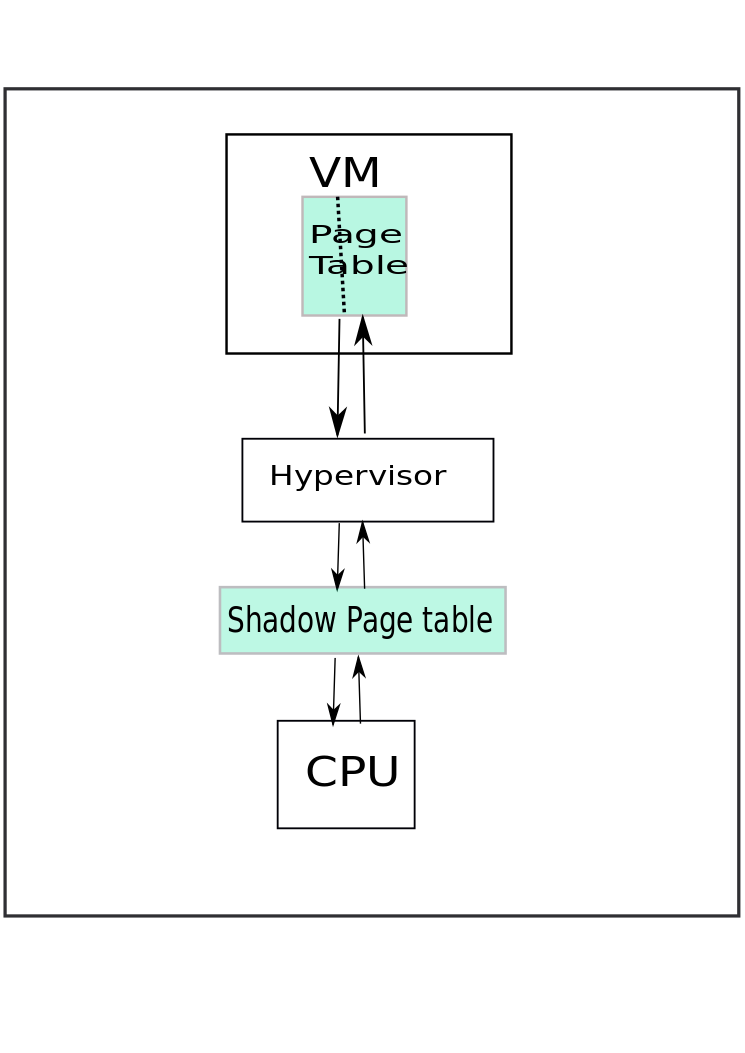
\includegraphics[scale =0.2]{shadow.png}
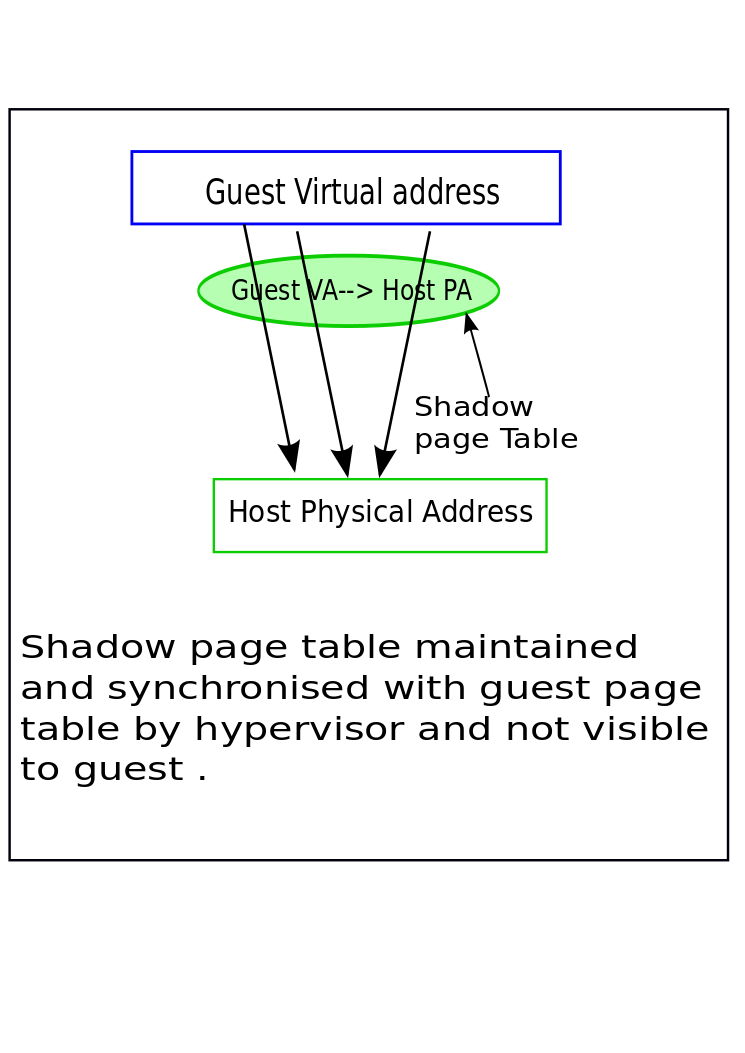
\includegraphics[scale =0.2]{page_table.png}
\caption{(a)Shadow page table architecture (b) Guest Address translation }
\end{figure}
\section{Comparison among Xen, KVM and other Virtualization technologies}
Xen and KVM are different from each other in architecture and features. Hardware support
was not available at the time when Xen released, so to implement some special operation in
guest OS which requires privilege and to reduce overhead Xen used paravirtualization but
now hardware support is available so Xen provides both configuration full virtualization
and paravirtualization. Difference in architecture: in Xen guests perform all network and
I/O operation with help of Dom 0, Dom 0 is a special guest to manage normal guests. 
Xen used privilege rings 1 and 2 for hypervisor and guests respectively to make privilege separate 
from kernel space and user space.
But KVM is like extension of Linux kernel so it uses Linux kernel architecture as a hypervisor
host and uses same Linux fair scheduler.
KVM uses one additional privelege level guest mode that is supported by hardware. 
For example: user can pin VM to a particular core by using normal Linux commands.\\
\begin{table}
\begin{center}
\label{tab-table}
\begin{tabularx}{\textwidth}{|X|X|X|}
%\begin{tabular}{|c|c|c|}
\hline
 Features & KVM & Xen \\
\hline
architecture& Bare metal & Hosted \\
\hline
scheduler& (process scheduler) Linux fair schedulers versions& (VM scheduler) SEDF, Credit\\
\hline
Network Management& FIFO based scheduling& FIFO based scheduling\\
\hline
Memory Address Translation& Shadow page table, Hardware Assisted Pagetable&Direct Pagetable, shadow page table, Hardware assited pagetable\\
\hline
\end{tabularx}
\caption {Properties of Xen and kvm\cite{xenkvm2014}}
\end{center}
\end {table}

\subsection{Description of experiment done to find performance related data.}
All experiments done with high performance computing system 
Linpack: to test execution speed by solving linear system of equations, PingPong Bandwidth: 
measures bandwidth of communication among CPU cores, Fast Fourier: measures the
speed of execution of DFT, ping pong latency: measures latency of communication among
CPU cores, SPEC OpenMP benchmark\cite{comparisonm}.
\subsection{Performance analysis}
High performance Computing KVM got the highest rating point according to \cite{comparisonm} and virtual 
box is very close to KVM, Xen left behind in rating. In ping pong bandwidth virtual
box shows results better than native because virtual box doesn’t pin its vcpu to a particular
hardware cpu so there is a case when two or more vm running on same physical cpu that
benefits in communication. Normal Performance system: In \cite{xenkvm2014} carried out some 
experiments CPU intensive, Memory intensive, Memory Bomb and conclude both KVM and Xen
performed approximately equal.
\section{Power Management in Virtualized Platforms}
Power management is directly related to hardware and frequency of cpu. Power management needs to communicate with hardware
directly but direct access rights to VM violates crucial properties of virtualization like
independence on hardware and isolation. So \cite{ripalm} provided nice solution for this VPM
states. VPM states also known as soft states, soft states are virtual version of p states provided by Intel and these
states are corresponding to performance To implement local power management at VM
level, VM continuously monitors utilization and according to that they requests desirable
soft state and these request for change in soft state sometimes can be simply ignored by
Dom0 to avoid control on hardware. All these request forwarded to Dom 0, with the help
of VM rules Dom0 takes appropriate action. VPM rule are rules and constraints to define
policies.
\subsection{Difference between Power Management and Virtual Power Management}
Difference between Power Management and Virtual Power Management
Datacentres use virtualization to make efficient use of hardware and for easy management 
of servers. In this scenario Power management at host level must be coordinated with VMs. 
Otherwise, it will lose opurtinities of global power management for ex. consolidation, 
so it need to track details about load on VMs and load on physical machine.
\subsection{Mechanisms to manage power in virtualized platform}
\subsubsection{Hardware Scaling}
In this strategy hardware support required, nowadays Intel hardware provides p states, p
stands for performance these states provides the range of states in which lower states are
high performance and consumes more power and higher states are corresponding to low
performance and low power consumption. These different states maintained by varying
frequency of CPU. So using this hardware support power management system can manage
power consumption by using appropriate p state according to current utilization of CPU.
\subsubsection{Soft Scaling}
When hardware support is limited for example cpu operate only on 2 or 3 different fre-
quencies so to make significant reduction power consumption there is need of range of
big range of p states. In this situation we can exploit scheduling process in hypervisor
to emulate more virtual p states, hypervisor scheduler can assign time slice according to
soft state of that VM For example if any VM requests to scale down frequency by 1/3 but
CPU does not operate on frequency/3 here we can use scheduler to emulate this situation
by assigning time slice which is one third of original time slice[6] There is a big draw
back in this approach that if a memory bound process gets less time slice then it affects
adversely because it is not equivalent to frequency scaling operation, if frequency scaling
available then memory bound process can get CPU for short period and goes back
to i/o operation but if time slice is reduced then it gets stuck waiting for CPU meanwhile
it could have done i/o instead of waiting for cpu, [6] does not provide effective solution for
this condition.
\subsubsection{Consolidation}
This method is most effective to reduce power consumption and it operates globally. A
central unit track all VMs load and tries to run VMs in a minimal set of hardware machine 
and turn down idle hardware machine. This strategy can be implemented easily by
keeping records and tracking VMs load and their Hardware machine’s load and search for
a machine which can accommodate more VMs simultaneously, if such Hardware machine
found using live migration feature Vm can move from one machine to other machine.
\subsubsection{Using C states}
[2] provided basic idea of this topic. When a system is idle it still consumes a lot power
and if goes for naive solution for this problem which is turn off idle systems then due to
frequent changes in states of system idle to busy, busy to idle. So its not feasible to turn off
system it will lead to drastic performance degradation because of large latency of turn on
a system. So we can opt second approach is a hardware support “C states”, c states stands
for core power states c0 is operating state other are non-executing states sleeping states
varies in degree of sleeping. Deeper states save more power but comes with drawback
long latency to switch back in executing mode. Actually these state implemented using
turn of clocks and timers which are running in idle state of cpu. There is a Challenge with
deeper c states. Deeper states turn off clocks and timer so there is problem of timer skew.
In this approach we can use tracking history of c states uses and prepare a c state plan
based on the prediction. This approach is effective in periodic type behavior\cite{cstates}.
\subsection{Power Consumption Reduction}
UUsing all above mechanism reduction in power consumption can be done effectively
all mechanism discussed above works on different for example Hardware Scal-
ing and Soft Scaling acts on local level with DVFS each VM tries minimize power con-
sumed. Consolidation works at global level which tracks VMs and physical machines
tries to accommodate max no. VMs on the minimal set of physical machine without
affecting performance. C states dealing with power consumption when cpu is idle. So
applying all these approaches we can reduce power consumption effectively.
.
%\subsection{How power consumption reduced and verification}

\section{Challenges related to virtual power management}
\subsection{ Different Purpose power management}
There are different power management which serves different goals. If a power demand goes high and it remains high then
there is risk of thermal fail-over which will destroy hardware this must not happen so
there should be a plan to avoid thermal fail-over even in overloaded situation\cite{nostruggle}.
%\subsection{Difference between Power Management at Local level and Global level}
%Local level power management rely on VMs and 
\subsubsection{Average Power Consumption}
This plan is to reduce average power consumption by using local and global power man-
agement.
\subsubsection{Power Capping}
This plan is to prevent thermal fail-over by restricting peak power consumption, as ob-
served running system on peak power for very short period does not lead to thermal fail-over, so a soft power management is fine.
\subsubsection{Power planning on the basis of history}
This plan works when behavior of load is periodic and predictable for such situation this plan try to ensure that CPUs
provide max resource as well as doesn't cross max peak power at the time of peak load, it can be done by a simple idea that 
before getting high load try to finish previous work by giving some extra power.
\subsection{Conflict among simultaneous Power Management for different Purpose and Coordination}
When two or more different power management trying to achieve different goals there is great chance of Inconsistency.
For example two power management plans working on same system one is for managing average power consumption and one is for managing
max power and power budget.
both power management can interfere each other by overwriting p states of system.
There is one more scenario in which problem created due to lack of coordination between Consolidation plan running at global level and
local power budget.
Consolidation plan may accommodate VMs on physical machine which violates power budget of that physical machine\cite{nostruggle}.\par
\begin{figure}[!htb]
\label{arch}
\label{fig-circles}
\centering
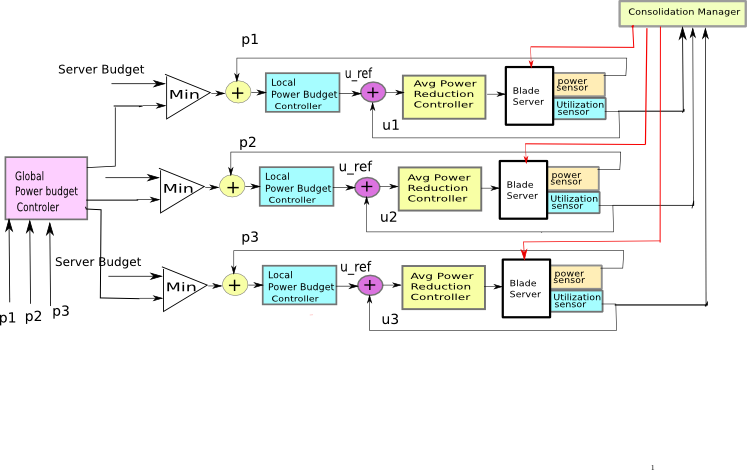
\includegraphics[scale =0.6]{arch.png}
\caption{Coordination architecture with blade server\cite{nostruggle}}
\end{figure}
Solution of conflicts between power management needs change in architecture and requires sensor, controller, feedback mechanism.
Power management can be implemented through controller and to prevent conflicts inputs provided to controller should filtered by comparator. 
In \label{arch} Consolidation Manager manages VM migration among Blade Servers, consolidation may violate local power budget by
migrating VMs to a particular Blade server, to avoid this situation Consolidation Manager keep track of local budget of each blade server.
Avg Power Reduction Manager controller compare Uref Ui to manage frequency of blade Server. Local Power Budget controller manages budget by
varying u\_ref. Global Power Budget controller works in a periodic manner, it recalculate and assign local power budget after each time interval.  
\subsection{Unfairness to some VM due to frequency scaling}
Lets take a Case of Service Provider and Consumer, assume there is no priority for any VM.
Consumer wants some computing resources (cpu) to run his/her VM but he wants to use a part of computation capacity so
there is Credit allocation scheme which defines how much of computing resources will be available to consumer VM for example 
40 credits means 40\% of computing resources available to VM provided that cpu frequency is max.
Consider provider wants to reduce power consumption so there is power management which is using DVFS (Dynamic voltage and frequency scalling)
DVFS monitors utilization of cpu in closed feedback loop if utilization becomes lower then it scale down frequency to reduce power 
consumption. Whenever frequency scaled down there are chances that some overloaded VM promised X credit computing resources getting 
less amount of computing resources than promised because now frequency is scaled down. This creates unfairness toward VMs.
\subsection{Introduction of different VM Scheduler}
\subsubsection{ Fixed credit scheduler}
In this type of VM scheduler if VM is promised X credit then VM will get at most X credit of computing resources even (Max credit-X) is unused and
idle, and VM will get time slice according to credit X always.
\subsubsection{ Variable credit scheduler}
In this type of VM scheduler if VM is promised X credit then VM will get X credit of computing resources provided that VM needs it
if VM is idle or it is underloaded then free computing resources will be distributed among other needy VM.
For example- Three VMs are running each allocated 33 credits. and Max credit is 99.
Two VMs are underloaded and one is overloaded then overloaded VM use free time slices made available by two underloaded VM, "free" time slice
means that two underloaded VM must get computing resources according to their need they must not suffer in terms of performance.
If all VM are at full utilization then all three VM will get promised computing resources No extra resources because computing resources is not free. 
Variable credit scheduler solves indirectly ``unfairness to VM'' problem but there is a drawback in this solution 
that is not desirable for service provider because unless all VM are underloaded or idle frequency scale down action can not be performed. 
There are very less chance to scale down frequency which results increased cost of power used, 
because power cost can not be minimized effectively in this case.
Ideal situation is when all VM gets computing resources as they promised always and 
and no chance to scale down frequency should be prevented due to providing extra free time slice. 
\subsubsection{ DVFS aware credit scheduler}
This scheduler considers both provider and consumer, this scheduler recompute credit of a VM on each frequency scale operation.
For example if one VM allocated 30 credits and max frequency is F, if frequency scaled down to F/2 then VM getting actually equivalent to 15 credits computing
resources so to make it equivalent to 30 credits at maximum frequency change credit 30 – 60. Now 60 credit with F/2 frequency is 
equivalent to 30 credits\cite{dvfs}.
\subsection{How can we avoid unfairness to VMs by making changes to scheduler}
As DVFS aware credit scheduler described above it is different from other schedulers because it focus on Actual credit.
Lets RC = ( credit x freq1) is real credit, if frequency decreases multiplicatively by factor d.

Now new frequency is freq1/d to keep RC constant credit should be multiplied by d, RC = (d x credit) x freq1/d 
now RC becomes again credit x freq1. This simple task need to be performed to avoid unfairness.\cite{dvfs}.
\section{Conclusion}
Growing demand of internet requires big cloud system and server farms.
To manage server farm and data centers easily and efficiently there is need of virtualization.
Power consumption is directly related to environment so we are responsible to use it efficiently. A good power management required.
Combination of virtualization and power management is more effective.

\addcontentsline{toc}{section}{References}
\bibliographystyle{plain}
\bibliography{reference}
\end{document}
%%% Local Variables: 
%%% mode: latex
%%% TeX-master: t
%%% End: 
